%% Spaghetti Architect — DMLR (Journal of Data-centric Machine Learning Research).
%% Target: data.mlr.press — the ROLLING ARCHIVAL JOURNAL (NOT the dmlr.ai ICLR/ICML
%% workshops, which are deadline-based). This is the fast, no-deadline resource paper.
%%
%% TEMPLATE TODO: data.mlr.press was unreachable at drafting time. Before submission,
%% swap this self-contained `article` preamble for the OFFICIAL DMLR/JMLR style
%% (jmlr/jmlr2e from the DMLR GitHub) and CONFIRM on the journal site:
%%   (1) exact length norm  — JMLR-family is flexible/paper-length, NOT the workshop's 8pp cap;
%%   (2) double-blind anonymization policy (anonymize author + the GitHub URL for review if so);
%%   (3) whether a reproducibility statement / Croissant record is wanted in-band.
%%
%% BUILD:  pdflatex dmlr -> bibtex dmlr -> pdflatex dmlr -> pdflatex dmlr
%%
%% SCOPE (read before editing): this is the DATA-CENTRIC RESOURCE paper — the generator
%% + the contamination-resistant, by-construction-labelled, multi-language code dataset
%% + label-validity evidence + reference baselines. It MUST NOT report the LLM-as-judge
%% meta-evaluation FINDINGS: that empirical study is the SEPARATE, deferred paper
%% (seed: bench/paper/benchmark.tex). Cite it only as a motivating use case; never put
%% its (unrun) numbers here.

\documentclass[11pt]{article}

\usepackage[T1]{fontenc}
\usepackage[utf8]{inputenc}
\usepackage{amsmath,amssymb}
\usepackage{booktabs}
\usepackage{graphicx}
\usepackage{xcolor}
\usepackage{tikz}
\usetikzlibrary{positioning,fit,backgrounds,shapes.geometric}
\usepackage{listings}
\usepackage[hidelinks]{hyperref}
\usepackage{url}
\usepackage{natbib}        % JMLR/DMLR uses natbib
\usepackage{geometry}
\geometry{margin=1in}
\usepackage{cleveref}  % load after hyperref; names references ("Section", "Table", ...) itself
\crefname{lstlisting}{Listing}{Listings}
\Crefname{lstlisting}{Listing}{Listings}
\crefname{appendix}{Appendix}{Appendices}
\Crefname{appendix}{Appendix}{Appendices}

\lstset{basicstyle=\ttfamily\small,breaklines=true,frame=single,columns=fullflexible}

% editorial markup — STRIP before camera-ready (a single \renewcommand to {} hides them)
\newcommand{\todo}[1]{\textcolor{red}{\textbf{[TODO: #1]}}}
\newcommand{\owner}[1]{\textcolor{blue}{\textsf{[\textbf{owner:} #1]}}}
\newcommand{\port}[1]{\textcolor{orange}{\textsf{[port: #1]}}}

\newcommand{\tool}{\textsc{Spaghetti Architect}}

\title{\tool: A Contamination-Resistant, By-Construction-Labelled,\\
       Multi-Language Code Dataset Generator}

\author{Kurath\\ \todo{affiliation / email --- confirm DMLR anonymity policy first}}
\date{}

\begin{document}
\maketitle

\begin{abstract}
\owner{PROSE --- refine this draft to $\sim$180 words, data-centric framing}
Mining-based code corpora are abundant but \emph{uncontrolled}: a snippet's semantics,
its surface ``messiness,'' and its difficulty are whatever the wild happened to
contain, there is no known-optimal reference to grade against, and any public sample
may already sit in a model's training set. We present \tool, a tool that mints code
datasets with exactly the control such corpora lack. An \emph{anti-optimization
transpiler} maps a clean, language-agnostic JSON intermediate representation to
deliberately redundant, fully-flattened programs in five languages
(Python, JavaScript, Go, Java, C++); every emitted program is compiled, run, and
checked against a reference oracle, so each instance is correct \emph{by construction}.
Because the clean IR is a known-optimal reference and ``messiness'' is dialed by
composable, strictly-nested anti-pattern profiles, the tool labels each instance along
two \emph{orthogonal} difficulty axes --- intrinsic (problem size) and incidental
(presentation at fixed semantics) --- and resists contamination by minting fresh
variants from a private held-out seed. We document the generator and the dataset it
produces, give construct-validity evidence that the by-construction quality order moves
established complexity and readability metrics, and report reference baselines. The
artifact is open source (MIT), dependency-free, and archived with a DOI.
\end{abstract}

%% sections/intro.tex
%% Data-centric (DMLR) framing: foreground value to ML research, not just SE tooling.

\section{Introduction}
\label{sec:intro}

Source code is one of the most heavily used data modalities in machine learning, and
the dominant way to obtain it is to mine it: scrape repositories, filter, deduplicate,
and ship. Mined corpora are abundant, but they are \emph{uncontrolled}. A snippet's
semantics, its surface ``messiness,'' and its difficulty are whatever the wild happened
to contain; there is no known-optimal reference to grade an instance against; and the
two things a study most often wants to vary --- \emph{how hard the problem is} and
\emph{how poorly it is written} --- are confounded, because in real code a longer
program is usually also a messier one. Worse, every public sample is a moving target for
contamination: any snippet a researcher uses to evaluate a code model may already sit in
that model's training set, so a high score can reflect memorization rather than
capability~\citep{contamination-placeholder}. Mining gives us volume; it does not give us
\emph{control}, \emph{labels}, or \emph{freshness}.

A growing set of data-centric ML problems need exactly that control. Contamination-aware
evaluation of code models requires items that can be \emph{re-minted} after a training
cutoff rather than drawn from a static, leakable pool. Training and probing studies want
parallel data in which one factor moves while the rest are held fixed. Robustness
analysis wants to ask whether a model degrades because \emph{the problem got bigger} or
because \emph{the presentation got messier} --- a question no fixed corpus can answer,
because the two grow together in the wild. Refactoring, clone-detection, and
code-translation research wants paired clean/messy programs whose semantic equivalence is
\emph{guaranteed}, not merely assumed from a commit message. Each of these is a request
for a piece of data that mined corpora structurally cannot supply: a labelled,
equivalence-controlled, freshly-mintable, multi-language instance.

We present \tool, a tool that synthesizes such data. \tool{} is an
\emph{anti-optimization transpiler}: where an optimizing compiler holds semantics fixed
and \emph{minimizes} a cost, \tool{} holds semantics fixed and deliberately
\emph{maximizes} incidental complexity. It maps a clean, language-agnostic JSON
intermediate representation (IR) to deliberately redundant, fully-flattened programs in
five languages (Python, JavaScript, Go, Java, C++), and every emitted program is
compiled, run, and checked against a reference oracle, so each instance is correct
\emph{by construction}. Because the clean IR is a known-optimal reference and
``messiness'' is dialed by composable, strictly-nested anti-pattern profiles, each
instance carries labels along two \emph{orthogonal} difficulty axes --- \emph{intrinsic}
(the problem genuinely grows) and \emph{incidental} (presentation degrades at fixed
semantics) --- and a single IR yields a parallel corpus across all five languages. To
resist contamination, scored instances are minted fresh from a \emph{private} held-out
seed that is never committed, a public canary GUID enables training-set audits, and
graded novelty tiers turn ``how memorized is this?'' into a measured quantity rather than
a hope. A motivating downstream use case --- a meta-evaluation of whether LLM judges
track a code-quality order known independently of any rater --- is the subject of a
separate, deferred study~\citep{TODO-companion-study}; here we deliver and document the
\emph{instrument} and the dataset it produces.

\paragraph{Contributions.} This paper contributes:
\begin{itemize}
  \item \textbf{The generator and its correctness-by-construction design}
        (Section~\Cref{sec:resource}): a staged IR$\rightarrow$five-language pipeline in which
        valid syntax is structural and runtime safety is always-on, gated by an oracle
        validator so that every released instance provably builds and computes the
        intended result.
  \item \textbf{Two orthogonal, by-construction difficulty labels}
        (Section~\Cref{sec:axes}): an \emph{incidental} messiness knob (a strictly-nested
        anti-pattern ladder) crossed with an \emph{intrinsic} problem-size knob, so a
        score change can be attributed to one cause with the other held fixed --- a
        decomposition no mined corpus offers.
  \item \textbf{A contamination protocol} (Section~\Cref{sec:contam}): mint-after-cutoff
        generation, a public \texttt{dev} split versus a private held-out \texttt{test}
        split, an embedded canary, and graded A/B/C novelty tiers --- with the
        public/private asymmetry as the mitigation, not an apology.
  \item \textbf{Construct-validity evidence} (Section~\Cref{sec:validity}) that the
        by-construction quality order moves established complexity and readability
        metrics, reported with its weaknesses stated plainly.
  \item \textbf{Reference baselines} (Section~\Cref{sec:baselines}) that establish the
        dataset is usable and discriminative, and a reusable, FAIR, DOI-archived,
        dependency-free open-source artifact.
\end{itemize}

\paragraph{Artifact.} \tool{} is open source under the MIT license, depends only on the
Python standard library, ships runnable examples, a test suite, and a documented
extension contract, and is archived with a DOI; a ``Datasheet for Datasets''
(Appendix~\Cref{app:datasheet}) accompanies the dataset.

%% sections/resource.tex
%% GOAL: describe the RESOURCE — the generator pipeline, the operation/
%% anti-pattern model, the two orthogonal difficulty axes, the oracle/validation, and the
%% contamination protocol.

\section{The Resource}
\label{sec:resource}

\subsection{Pipeline overview}
\tool{} is a staged pipeline that turns a clean, language-agnostic JSON IR into an
oracle-validated, two-axis-labelled multi-language dataset (\Cref{fig:pipeline}).

\begin{figure}[t]
\centering
\resizebox{\linewidth}{!}{%  scale the picture to fit the (narrower) DMLR column width
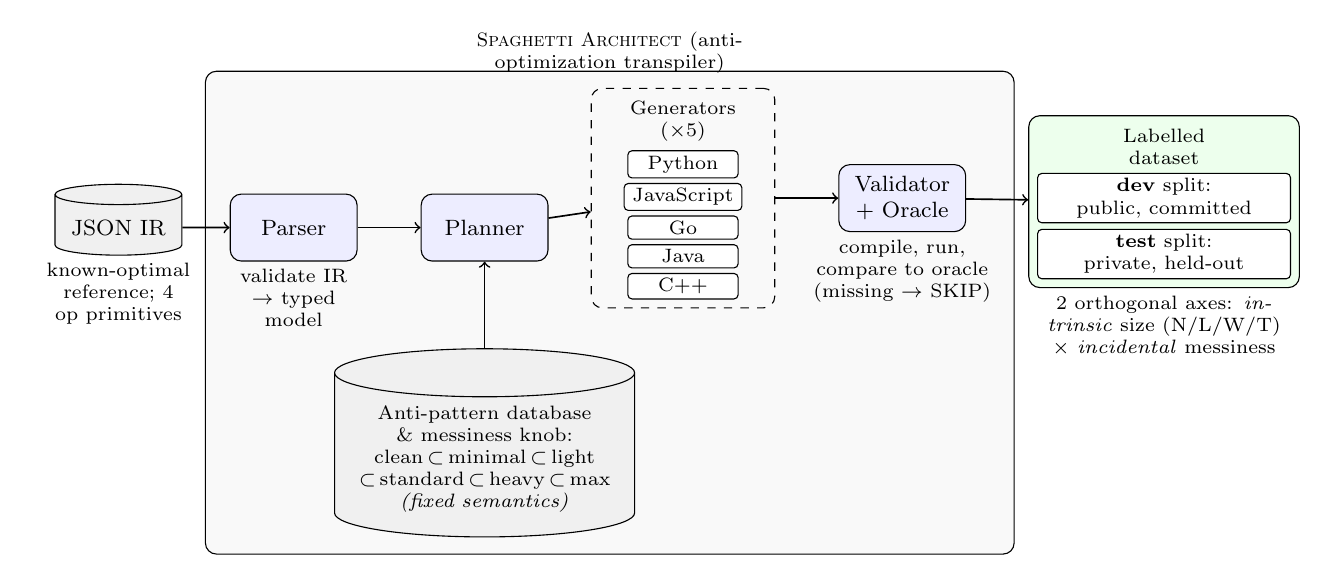
\begin{tikzpicture}[
  font=\footnotesize,
  node distance=5mm and 6mm,
  every node/.style={align=center},
  stage/.style={draw, rounded corners, fill=blue!7, inner sep=3pt, minimum height=8.5mm, text width=14mm},
  store/.style={draw, cylinder, shape border rotate=90, aspect=0.16, fill=gray!12, inner sep=3pt, minimum height=9mm, text width=14mm},
  chip/.style={draw, rounded corners=1.5pt, fill=white, inner xsep=3pt, inner ysep=1.8pt, font=\scriptsize, minimum width=14mm},
  note/.style={font=\scriptsize, inner sep=1.5pt, text width=20mm},
  flow/.style={->, semithick},
]
% input
\node[store] (ir) {JSON IR};
\node[note, below=1pt of ir, text width=22mm] (ops) {known-optimal reference; 4 op primitives};
% parser
\node[stage, right=of ir] (parser) {Parser};
\node[note, below=1pt of parser, text width=17mm] (pnote) {validate IR $\to$ typed model};
% planner
\node[stage, right=8mm of parser] (planner) {Planner};
% generators
\node[chip, right=10mm of planner] (g3) {Go};
\node[chip, above=1.6pt of g3] (g2) {JavaScript};
\node[chip, above=1.6pt of g2] (g1) {Python};
\node[chip, below=1.6pt of g3] (g4) {Java};
\node[chip, below=1.6pt of g4] (g5) {C++};
\node[note, above=1.4pt of g1] (genlbl) {Generators ($\times5$)};
\node[draw, rounded corners, dashed, fill=none, inner sep=3pt, fit=(genlbl)(g5)] (gen) {};
% validator
\node[stage, right=8mm of gen] (val) {Validator\\+ Oracle};
\node[note, below=1pt of val, text width=23mm] (vnote) {compile, run, compare to oracle (missing $\to$ SKIP)};
% anti-pattern database / messiness knob feeding the planner
\node[store, below=11mm of planner, text width=36mm, font=\scriptsize] (db)
  {Anti-pattern database \& messiness knob:\\clean\,$\subset$\,minimal\,$\subset$\,light\\$\subset$\,standard\,$\subset$\,heavy\,$\subset$\,max\\\textit{(fixed semantics)}};
% output splits
\node[chip, right=9mm of val, text width=30mm] (dev) {\textbf{dev} split:\\public, committed};
\node[chip, below=2pt of dev, text width=30mm] (test) {\textbf{test} split:\\private, held-out};
\node[note, above=1.4pt of dev] (datalbl) {Labelled dataset};
% background fills (drawn behind node contents so labels stay visible)
\begin{scope}[on background layer]
\node[draw, rounded corners, fill=green!7, inner sep=3pt, fit=(datalbl)(dev)(test)] (data) {};
\node[draw, rounded corners, fill=gray!5, inner sep=6pt, fit=(parser)(pnote)(planner)(gen)(val)(vnote)(db)] (tool) {};
\end{scope}
% flow
\draw[flow] (ir) -- (parser);
\draw[flow] (parser) -- (planner);
\draw[flow] (planner) -- (gen);
\draw[flow] (gen) -- (val);
\draw[flow] (val) -- (data);
\draw[flow] (db) -- (planner);
% annotations
\node[note, text width=40mm] at ([yshift=2.3mm]tool.north) {\tool{} (anti-optimization transpiler)};
\node[note, below=1pt of data, text width=34mm] (axes) {2 orthogonal axes: \emph{intrinsic} size (N/L/W/T) $\times$ \emph{incidental} messiness};
\end{tikzpicture}%
}% end \resizebox
\caption{The \tool{} pipeline. A clean, language-agnostic JSON IR---built from four
operation primitives (\texttt{MEMBERSHIP\_CHECK}, \texttt{KEY\_VALUE\_LOOKUP},
\texttt{AGGREGATE}, \texttt{CONDITIONAL\_SELECT}) and serving as the known-optimal
reference---is validated by the \emph{Parser} into a typed model, so a malformed IR can
never reach a generator. The \emph{Planner} then selects an anti-pattern profile from a
data-driven database via the strictly-nested six-level messiness knob
(\textsf{clean} $\subset$ \textsf{minimal} $\subset$ \textsf{light} $\subset$ \textsf{standard} $\subset$ \textsf{heavy} $\subset$ \textsf{max})
\emph{at fixed semantics}; five \emph{Generators} emit the deliberately redundant,
fully-flattened programs (Python, JavaScript, Go, Java, C++); and the \emph{Validator}
compiles and runs each target against a reference \emph{oracle} (a missing toolchain
\textsf{SKIP}s, never a silent pass). The output is a dataset labelled along two
orthogonal difficulty axes---\emph{intrinsic} problem size ($N$/$L$/$W$/$T$) and
\emph{incidental} presentation (the messiness knob at fixed semantics)---split into a
public, committed \texttt{dev} split and a private \texttt{test} split minted from a
never-committed held-out seed.}
\label{fig:pipeline}
\end{figure}

The \emph{Parser} validates the IR into a typed model (so a malformed IR can never reach
a generator). The \emph{Planner} reads a data-driven anti-pattern database and selects
which transforms apply per operation at the chosen \emph{profile}. Each of five
\emph{Generators} emits source through a \texttt{CodeEmitter} that makes correct
indentation/bracing \emph{structural} rather than hand-managed, with always-on safety
(try/catch + guards + a pre-set fallback) injected via hooks. The \emph{Validator}
compiles and runs each target and compares its output to a reference \emph{oracle}.

\paragraph{Design properties.}
\begin{itemize}
  \item \emph{Correctness by construction.} Valid syntax is structural; safety is always
        on, so output is crash-free regardless of profile strength.
  \item \emph{Provable correctness.} Every target is compiled, run, and checked against
        the oracle; a missing toolchain \textsf{SKIP}s (never a silent pass).
  \item \emph{Deterministic.} The same IR yields byte-identical output (enabling
        golden-snapshot testing and reproducible datasets).
  \item \emph{Data-driven.} The anti-patterns and strength profiles live in a JSON
        database, not in code.
\end{itemize}

\subsection{Operations and anti-patterns}
\label{sec:ops}
The IR composes a sequence of typed \emph{operations} (Table~\ref{tab:ops}); each reads
validated inputs and writes a fresh result variable.

\begin{table}[t]
\centering
\caption{Supported operations (v0.2).}
\label{tab:ops}
\begin{tabular}{@{}lll@{}}
\toprule
Operation & Semantics & Result \\
\midrule
\texttt{MEMBERSHIP\_CHECK}   & \texttt{target in collection}              & bool \\
\texttt{KEY\_VALUE\_LOOKUP}  & \texttt{map.get(key, default)}             & scalar \\
\texttt{AGGREGATE}           & \texttt{sum|min|max(int collection)}       & int \\
\texttt{CONDITIONAL\_SELECT} & \texttt{then if (a$\,\bowtie\,$b) else else}& scalar \\
\bottomrule
\end{tabular}
\end{table}

The eleven \texttt{SPAGH\_*} transforms span structural, verbosity, control, and layout
categories; three are grounded in the Collberg--Thomborson obfuscation
taxonomy~\citep{collberg1997taxonomy} and classic code smells~\citep{fowler-refactoring}.
They compose into three strictly-nested profiles
(\textsf{minimal}~$\subset$~\textsf{standard}~$\subset$~\textsf{max}); the released
dataset uses a finer six-level knob
(\textsf{clean}~$\subset$~\textsf{minimal}~$\subset$~\textsf{light}~$\subset$~\textsf{standard}~$\subset$~\textsf{heavy}~$\subset$~\textsf{max})
in which each level adds transforms without removing any, so that set inclusion is the
order. The four categories are: \emph{structural} (replace a built-in with a manual
index loop; reorganize control flow), \emph{verbosity} (introduce intermediate variables
and redundant assignments), \emph{control} (opaque predicates that are provably constant,
de-hoisted recomputation, Yoda-style comparisons), and \emph{layout} (indentation and
bracing changes that the \texttt{CodeEmitter} renders structurally). Each backend lowers
the same transform idiomatically; only C++ emits genuine pointer arithmetic for the
manual-index pattern.

\Cref{lst:ir} and~\Cref{lst:spag} show the contrast for a single \texttt{MEMBERSHIP\_CHECK}: a
four-line IR fragment and an excerpt of the Python the \textsf{max} profile emits from it.
The clean reference is the membership test \texttt{search\_val in data\_list}; the
\textsf{max} render computes the same boolean through a manual index loop, a de-hoisted
\texttt{len()} call, an always-true opaque predicate, and an always-on
\texttt{try}/\texttt{except} fallback. The semantics are identical; only the incidental
complexity differs.

\begin{lstlisting}[caption={IR fragment for one \texttt{MEMBERSHIP\_CHECK} operation.},label={lst:ir},basicstyle=\ttfamily\footnotesize]
{"operation": "MEMBERSHIP_CHECK",
 "collection_name": "data_list",
 "target_var": "search_val",
 "result_var": "is_found"}
\end{lstlisting}

\begin{lstlisting}[language=Python,caption={The \textsf{max}-profile Python emitted from Listing~\ref{lst:ir} (verbatim; comments are the tool's own anti-pattern annotations).},label={lst:spag},basicstyle=\ttfamily\footnotesize]
is_found = False
try:
    if data_list is not None:
        # SPAGH_001/006/008: manual index loop instead of `in`
        _idx = 0
        # SPAGH_010: recompute len() every iteration (de-hoisted)
        _match_flag = False
        while _idx < len(data_list):
            _current = data_list[_idx]
            # SPAGH_009: opaque predicate (always true: n*(n+1) is even)
            if (_idx * (_idx + 1)) % 2 == 0:
                if search_val == _current:
                    _match_flag = True
                else:
                    _match_flag = _match_flag
            _idx = _idx + 1
        is_found = _match_flag == True
    else:
        is_found = False
except Exception:
    is_found = False
\end{lstlisting}

\subsection{Two orthogonal difficulty axes}
\label{sec:axes}
A dataset can vary \emph{intrinsic} complexity (the problem genuinely grows: cascade
arms, list length, operation count) independently of \emph{incidental} complexity (the
\textsf{clean}$\rightarrow$\textsf{max} profile adds mess at \emph{zero} semantic change).
This separation, which no fixed mined corpus offers, lets a study ask whether a
method fails because the \emph{problem} got bigger or because the \emph{presentation} got
messier. The incidental axis is the dataset's by-construction quality order: a strict
nesting that holds independently of any rater.

In mined corpora the two axes
are \emph{confounded}: a longer program is usually also a messier one, so size and
presentation cannot be moved independently. \tool{} instead crosses them fully (every
base sample is rendered at every messiness level), so the incidental knob carries no
information about problem size. Over the public \texttt{dev} split this is exact: the
Spearman correlation between the messiness-knob rank and two presentation-independent
intrinsic-size measures --- the IR operation count and the per-family scale knob
($N/L/W/T$) --- is $\rho = 0.00$ across all $250$ (base sample, profile) cells, and
$\rho = 0.00$ within each family whose scale knob varies (computed in
\texttt{bench/anchor.py}, recorded in \texttt{anchor.json}). The two difficulty axes are
therefore orthogonal by construction \emph{and} verified balanced in the release. Nor
is the intrinsic axis cosmetic: sweeping it alone collapses the exact-match
accuracy of even the strongest model we tested on the aggregation family to zero
(\Cref{sec:baselines}, \Cref{tab:scaling}), evidence that the size knob controls genuine
difficulty, not just token count.

The same intrinsic sweep separates two competences on \emph{identical}
programs. As the aggregation width $W$ grows over the same \texttt{agg\_stats} samples,
comprehension exact match collapses (the model must compute the sum) while refactor
equivalence (\texttt{semantic\_ok}) stays high and width-invariant (the model need only
restructure). On the same inputs the dataset thus isolates a \emph{computational}
competence from a \emph{structural} one (\Cref{sec:baselines}).

\subsection{Contamination protocol}
\label{sec:contam}
A public generator is defensible for contamination-aware evaluation provided every
\emph{scored} instance is minted \emph{after} a model's training cutoff. The defense is
the \emph{protocol}, not the artifact, so we make no ``contamination-proof'' claim; what
we provide is a structural asymmetry that keeps the scored data fresh.

\paragraph{Public \texttt{dev} versus private held-out \texttt{test}.} The dataset ships
in two splits minted from one generator. The \texttt{dev} split is \emph{public}: it is
committed to the repository so that the format, the labels, and the pipeline are fully
inspectable and reproducible. Because a public split can itself leak into
future training sets over time, the scored \texttt{test} split is \emph{private}: it is
minted from a secret seed (\texttt{BENCH\_HELDOUT\_SEED}, an environment variable that is
never committed) by re-drawing every numeric literal and salting string literals, and is
excluded from version control. Anyone with the released generator can regenerate an
equivalent private split from their own fresh secret seed --- so the
\emph{mint-after-cutoff} guarantee survives even after the public split is fully
absorbed. The asymmetry is the mitigation: the inspectable half is allowed to be
trainable so that the scored half does not have to be.

\paragraph{The freshness guarantee, measured.} The protocol's premise --- that the private
split is a faithful, un-memorized re-mint of the public one --- is itself testable. Across the four-model reference ladder (\Cref{sec:baselines}), comprehension exact
match on the public \texttt{dev} split equals exact match on the private Tier-A
\texttt{test} split to within $|\Delta|\le 0.012$ per model, and refactor
\texttt{semantic\_ok} agrees between \texttt{dev} and Tier-A \texttt{test} across the
ladder ($|\Delta|\le 0.011$; DeepSeek-V4-Flash $\Delta=-0.0001$). Because every \texttt{test} prompt hash
differs from its \texttt{dev} counterpart, the agreement reflects preserved difficulty
under a full re-mint of the scored literals, not reuse: the contamination-resistance
property is thus measured.

\paragraph{Canary.} A canary GUID --- a unique, memorizable string in the spirit of the
unintended-memorization probes of \citet{carlini2019secret} --- is embedded in the public
release (\texttt{spaghetti-architect-bench:\allowbreak canary:\allowbreak 9f1d4e7a-\dots}).
A model that reproduces it has demonstrably ingested the public split, turning training-set
inclusion into something an auditor can probe rather than assume.

\paragraph{Graded contamination-resistance tiers.} Freshness is not binary, so we
regenerate held-out structure at three tiers, each defeating a distinct mode of
memorization; these tiers are a contamination-resistance mechanism (regenerable
held-out splits), not a generalization or novelty probe. \textbf{Tier A} (literal-novel)
re-mints numeric literals and salts strings, defeating verbatim memorization. \textbf{Tier
B} (structural held-out) keeps the operation-chain \emph{shapes} private, defeating
memorization of structure. \textbf{Tier C} (scale/depth held-out) uses deeper chains and
out-of-range scales, regenerating structures outside the public split's scale and depth
range so they cannot have been memorized verbatim. What the tiers certify is freshness,
not generalization: the across-tier accuracy differences are \emph{operation-count
composition} (Tier~A is over half single-operation items, of which Tier~B has none) plus
the \texttt{agg\_stats} computation tax (\Cref{sec:baselines}), not a novelty penalty.
Directly standardizing Tier~A's exact match onto Tier~B's operation-count distribution
shrinks the mean Tier-A$-$Tier-B gap by $60$--$90\%$ across all four reference models and
\emph{reverses} its sign at the shared three-operation stratum, where Tier~B is the more
accurate tier; the full per-(tier, operation-count) and per-(tier, family) decompositions
are released in the analysis artifact (\texttt{g3\_analysis.json}). Consistent with this, clean
controls that hold operation type fixed (out-of-range scale on lookups and membership,
out-of-range depth on conditional cascades) show essentially no degradation. The
contamination signal is instead the \emph{matched} comparison: re-minting the same
structures with fresh secret values leaves scores unchanged (\Cref{sec:baselines}). The held-out seed and the Tier B/C
structures are deliberately withheld; this is a contamination trade-off, not an omission,
and every minted IR --- public or held-out --- is re-validated by the parser before use.

%% sections/validity.tex
%% \owner{ANCHOR subagent}  GOAL: fill REAL construct-validity numbers and an honest
%% reading of them. Currently the committed bench/out/anchor.json has radon/lizard/
%% cognitive as SKIP (only Buse--Weimer ran, aggregate Spearman ~0.39). The subagent must:
%%   1. Run anchor.py in the quarantined venv so radon/lizard/cognitive are REAL:
%%        python3 -m venv /tmp/anchorvenv
%;        /tmp/anchorvenv/bin/pip install radon lizard cognitive_complexity
%%        /tmp/anchorvenv/bin/python bench/anchor.py    # -> bench/out/anchor.json
%%   2. Extract the headline numbers (Spearman of each metric vs the incidental knob rank)
%%      and fill Table~\ref{tab:validity} below.
%%   3. Write the honest reading: complexity metrics (radon/lizard CC) move strongly with
%%      the knob BUT that is partly BY CONSTRUCTION (the knob is built to inflate them);
%%      the less-tautological readability signal (Buse--Weimer features) is WEAKER
%%      (aggregate ~0.39) and a human-calibrated readability study is future work. Do NOT
%%      overclaim. This honesty is itself a selling point for a data paper.

\section{Construct Validity: do the labels mean anything?}
\label{sec:validity}

The by-construction quality order is only useful if it tracks quantities the community
already trusts. We test whether the incidental knob moves established static metrics
monotonically, over the public \texttt{dev} set ($50$ base samples expanded to $300$
sources across the six knob levels). For each base sample we hold semantics fixed and
compute Spearman's $\rho$ between the knob rank
(\texttt{clean}${}\prec{}$\texttt{minimal}${}\prec{}$\texttt{light}${}\prec{}$%
\texttt{standard}${}\prec{}$\texttt{heavy}${}\prec{}$\texttt{max}) and each metric,
reporting the mean over samples (Table~\ref{tab:validity}). The anchor tools
(\texttt{radon}~6.0.1, \texttt{lizard}~1.23.0, \texttt{cognitive\_complexity}~1.3.0)
are kept off the zero-dependency core and run only inside a quarantined virtualenv; a
missing tool records an honest \texttt{SKIP} rather than a fabricated number.

\begin{table}[t]
\centering
\caption{Spearman correlation between the incidental ``messiness'' knob rank and
established static metrics, averaged over the $50$ \texttt{dev} base samples (higher
$|\rho|$ = the label order is better reflected). Complexity metrics move strongly with
the knob, but partly \emph{by construction}; the less tautological readability signal is
markedly weaker.}
\label{tab:validity}
\begin{tabular}{@{}llr@{}}
\toprule
Metric (tool) & Direction & Spearman $\rho$ vs.\ knob \\
\midrule
Cyclomatic complexity (radon)        & + & $+0.75$ \\
Cyclomatic complexity (lizard)       & + & $+0.75$ \\
Cognitive complexity                 & + & $+0.80$ \\
Maintainability index (radon)        & $-$ & $-0.79$ \\
Buse--Weimer surface density (agg.)  & + & $+0.39$ \\
\bottomrule
\end{tabular}
\end{table}

\paragraph{Complexity moves strongly, but read this with care.}
The complexity anchors agree and move sharply with the knob: cyclomatic complexity
(identical at $\rho=+0.75$ under both \texttt{radon} and \texttt{lizard}), cognitive
complexity ($\rho=+0.80$), and the maintainability index in the expected
\emph{opposite} direction ($\rho=-0.79$). Two independent tool families converging on
the same ordering, and our own stdlib metric lane cross-checking against them at
$\rho>0.97$, is reassuring evidence that the labels are not arbitrary. We deliberately
under-claim here, though, because this agreement is partly \emph{tautological}: the
incidental knob is engineered to inject redundant control flow, dead branches, and
nested scaffolding, which is precisely what cyclomatic and cognitive complexity count.
A metric rising when we add the very constructs it was designed to detect confirms that
the transformation does what it says, but it is weaker evidence that the order matches
\emph{human} judgments of quality.

\paragraph{The readability signal is real but weaker; human calibration is future work.}
The more informative test is therefore the one anchor that is \emph{not} a complexity
counter. Our re-implementation of the Buse--Weimer~\citep{buse2010readability} surface
readability feature set (computed with the Python stdlib over the same sources)
correlates with the knob at only $\rho=+0.39$ in the documented density aggregate ---
roughly half the strength of the complexity metrics. We read this honestly: the knob
makes code denser and harder to read, but far less unambiguously than it inflates
control-flow complexity, and even this number is a surface-density proxy rather than the
original trained readability classifier (whose coefficients are not available offline,
so that anchor remains a recorded \texttt{SKIP}). The benchmark's construct validity
thus rests on convergent static evidence, not on a claim of calibrated human
readability. A fresh human-rated readability study aligned to this exact stimulus set is
the natural next step and is left as explicit future work; until then we treat the
$\rho=+0.39$ readability signal, not the $\rho=+0.80$ complexity signal, as the
conservative bound on how much the by-construction order reflects perceived quality.

%% sections/baselines.tex
%% GOAL: a "reference baselines" section showing the benchmark is usable and
%% discriminative, assembled from ZERO/LOW-COST data only:
%%   - the non-LLM baseline panel: clean-ceiling, rule-based, metric-heuristic judge
%;        python3 bench/run_bench.py --baselines     (real, no API)
%%   - ONE real model row from the already-collected DeepSeek partial:
%;        bench/out/subagent/{comprehend,refactor}__deepseek-v4-flash__*.json
%% Frame these as REFERENCE baselines for a resource — NOT as the meta-evaluation study
%% (that is the deferred paper). The model panel is illustrative/partial.
%% Numbers below are from bench/run_bench.py --baselines (dev split, all 7 families,
%% 5 languages) and the stored DeepSeek-v4-flash raw outputs (graded offline, no API).

\section{Reference Baselines}
\label{sec:baselines}

To show the dataset is usable and discriminative we report reference scores from
non-learned baselines plus one illustrative model. These are \emph{reference points for a
resource}, not a model evaluation; the full LLM study is separate, deferred work. All
numbers are on the public \texttt{dev} split (100 instances, 7 families, 5 languages,
$k{=}8$ samples). The non-learned panel is produced by \texttt{run\_bench.py
-{}-baselines} (pure standard library, zero API); the model row is computed offline from
already-collected DeepSeek-v4-flash raw outputs and is therefore \emph{partial and
illustrative}.

\begin{table}[t]
\centering
\caption{Reference baselines on the public \texttt{dev} split. Each cell states the
metric for the task it applies to; ``---'' marks a (task, baseline) pair for which no
baseline is defined (e.g.\ there is no rule-based output predictor for comprehension, and
the metric-heuristic judge is judge-only). \textbf{Refactor} is the semantic-gated
simplification-quality (fraction of the spaghetti$\rightarrow$clean gap closed, capped at
the clean floor) on the rigorous Python AST/MI lane ($n{=}300$ Python items); the
language-agnostic \texttt{uniform\_lane} (lizard cyclomatic complexity + token size +
Buse--Weimer surface density) gives $0.95$ across all five languages for the clean-ceiling.
\textbf{Judge} is position-swap--controlled pairwise accuracy over $n{=}250$ judge items
(all families/languages). \textbf{Comprehend} is output-prediction exact match. The
DeepSeek-v4-flash row is a single open model over a \emph{subset} of families, included
to show the metrics move on real model outputs --- not a model comparison.}
\label{tab:baselines}
\begin{tabular}{@{}lccc@{}}
\toprule
Baseline & Refactor & Judge (pairwise acc.) & Comprehend (EM) \\
\midrule
Clean-ceiling          & $0.83$ & ---    & ---    \\
Rule-based             & $0.00$ & ---    & ---    \\
Metric-heuristic judge & ---    & $0.99$ & ---    \\
DeepSeek-v4-flash (partial) & $0.61^{\dagger}$ & n/a$^{\ddagger}$ & $1.00^{\S}$ \\
\bottomrule
\end{tabular}

\vspace{2pt}
{\footnotesize
$^{\dagger}$ Python AST lane, \texttt{discovery\_pipeline} family only ($n{=}12$ graded
Python items; semantic-equivalence rate $0.76$ over all five languages of that family).
$^{\ddagger}$ No judge batch was collected for this model.
$^{\S}$ Pooled over the two collected families (\texttt{discovery\_pipeline},
\texttt{status\_router}); $160$ graded items.
\par}
\end{table}

The non-learned panel brackets the refactor task. The \emph{clean-ceiling} --- the
engine's own idiomatic clean rendering, graded through the same semantic gate and
metric as a model --- reaches $0.83$ AST simplification-quality (Python) and $0.946$ on
the language-agnostic uniform lane across all five languages, with a $1.00$
semantic-equivalence rate, and lands inside the optimality band on every item, confirming
the labelled optimum is reachable in every backend and the metric is not saturated at $1.0$. At the other
end, two non-learned references both score $0.00$: a pure autoformatter (lower bound;
semantics-preserving but removes no anti-patterns) and a conservative AST
\emph{rule-based} simplifier (constant-folding and literal dead-branch removal). Both stay
semantically correct yet recover essentially none of the construction gap, so the task is
non-trivial and demands genuine restructuring rather than reformatting. For the judge
task, the \emph{metric-heuristic judge} --- picking the lower static-complexity candidate
of each pair --- attains $0.99$ position-consistent pairwise accuracy (Spearman
rank-vs-complexity $\rho \approx -0.99$). This is a deliberately strong non-LLM reference:
because complexity is monotone with the construction knob \emph{by design}, any useful LLM
judge must be measured \emph{against} this floor, not merely above chance. Finally, the
DeepSeek-v4-flash row shows the metrics respond to real model outputs --- partial recovery
on refactoring ($0.61$, with $0.76$ of completions semantically valid) and saturated
exact-match on these small-output comprehension items ($1.00$) --- without constituting a
model evaluation. A bounded-cost strengthening (one or two additional cheap models across
all families, gated behind the live-run cost controls) is left to the deferred study if
reviewers want cross-model spread.

%% sections/related.tex
%% Data-centric (DMLR) related work. Land the four differentiators.

\section{Related Work}
\label{sec:related}

We position \tool{} as a \emph{data resource} against four neighboring lines of work:
data-documentation norms, code/LLM benchmarks and the contamination problem, and the
controlled-transformation literature (obfuscation, code smells, readability) from which
the generator borrows its primitives.

\paragraph{Data documentation.} The data-centric ML community has converged on
structured documentation of provenance, composition, and intended use: Datasheets for
Datasets~\citep{gebru2021datasheets} and Data
Cards~\citep{pushkarna2022datacards} ask a dataset's authors to make its construction and
limitations legible. We follow that norm rather than extend it: the dataset ships with a
datasheet (Appendix~\Cref{app:datasheet}). What is unusual here is that, because the data is
\emph{synthesized} from a documented generator rather than collected, the answers to
many datasheet questions (how instances were labelled, whether they were preprocessed,
whether they can be regenerated) are exact and machine-checkable rather than
best-effort recollections.

\paragraph{Code and LLM benchmarks, and contamination.} Functional-correctness
benchmarks such as those built around \textsc{HumanEval}-style
suites~\citep{chen2021evaluating} grade \emph{what} a model produces but fix
\emph{presentation} and, being static and public, are exposed to training-set
contamination~\citep{contamination-placeholder}: a model may score well because it has
seen the items. Two structural responses exist in the data-resource literature. One is to
gate on time and protect the scored portion of a release; the other is to make instances
\emph{regenerable} so that a fresh, never-seen draw is always available. \tool{} adopts
both --- a private held-out split minted after the cutoff plus a public canary
(Section~\Cref{sec:contam}) --- but, unlike a static suite, it is a \emph{generator}: the scored
data is not a fixed file to be protected but a fresh sample to be minted, which is the
only durable defense once a public split inevitably leaks.

\paragraph{Controlled code transformation.} The moves \tool{} composes are not new in
isolation. Source obfuscation deliberately degrades readability while preserving
behavior; the eleven \texttt{SPAGH\_*} transforms descend from the Collberg--Thomborson
taxonomy of obfuscating transformations~\citep{collberg1997taxonomy} (opaque predicates,
redundant computation) and from classic code smells~\citep{fowler-refactoring}. Code
readability has its own measurement tradition, most influentially the learned
surface-feature metric of Buse and Weimer~\citep{buse2010readability}, which we re-use as
an external validity witness (Section~\Cref{sec:validity}). The defining difference is one of
\emph{purpose and labelling}. An obfuscator emits degraded code but no quality
\emph{order} and no known-optimal target; a code-smell injector or a mutation tool
perturbs a program but (in the mutation case) deliberately \emph{breaks} semantics rather
than preserving them; a readability metric scores existing code but does not generate a
graded corpus. \tool{} reuses these primitives as a \emph{maintainability-degradation
knob with ground truth}: a strictly-nested ladder that is, by construction, a quality
order at fixed semantics.

\paragraph{The four differentiators.} Each neighbor supplies some of the affordances a
data-centric study needs; none supplies all four at once.
\begin{itemize}
  \item \emph{Oracle-verified semantic equivalence.} Every instance --- and, for the
        refactoring use case, every candidate rewrite --- is compiled, run, and checked
        against a reference oracle, so equivalence is established by execution rather than
        assumed from provenance. Obfuscators and smell injectors typically assert
        equivalence; mutation tools invert it.
  \item \emph{By-construction graded quality order.} The incidental knob is a
        strictly-nested anti-pattern inclusion chain, so the messy$\rightarrow$clean order
        is known \emph{independently of any rater}. Obfuscators give a binary
        clean/obfuscated contrast; readability metrics give a rater-dependent score, not a
        ground-truth order.
  \item \emph{Multi-language parallel corpus.} One IR emits the same logic in five
        languages, yielding aligned cross-language instances. Obfuscation and mutation
        tools are typically single-language.
  \item \emph{Contamination control.} Mint-after-cutoff generation with a private
        held-out split, a canary, and graded novelty tiers (Section~\Cref{sec:contam}). Static
        benchmarks and the transformation tools carry no contamination protocol.
\end{itemize}
\noindent To our knowledge no prior generator combines oracle-verified equivalence, a
by-construction graded quality order, a multi-language parallel corpus, and a
contamination protocol in a single artifact; that combination is the resource's novelty.

%% sections/limitations.tex
%% Honest Limitations & Ethics (ML-venue norm).

\section{Limitations and Ethics}
\label{sec:limits}

\paragraph{Scope of the generator.} The IR targets composable sequences of the four
operations in \Cref{tab:ops}, not arbitrary control flow, and
\texttt{AGGREGATE}/\texttt{CONDITIONAL\_SELECT} are restricted to integer operands. This
is a deliberate trade rather than an accident: integer-only results format
byte-identically across all five backends, which is what lets a single oracle check
equivalence across Python, JavaScript, Go, Java, and C++. Generated artifacts are
single-file programs, not repository-scale projects. Consequently the dataset is a
\emph{controlled stimulus}, and we claim findings about behavior on that stimulus ---
robustness to incidental complexity, equivalence-preserving transformation --- not that
absolute results transfer to real-world codebases. Scaling the instance count does not
widen this scope; broadening the operation set, the operand types, and the program
granularity is future work.

\paragraph{The readability leg of construct validity is weak.} The label order is
validated, not asserted (\Cref{sec:validity}), but the legs of that validation are
uneven. The complexity metrics move strongly with the knob, yet that is partly
\emph{by construction}: the same transforms that define a higher knob level (e.g.\ adding
a branch) mechanically inflate cyclomatic complexity, so those metrics are convergent but
not independent witnesses. The genuinely more independent leg is readability, and it is
weak: the surface-feature aggregate correlates with the knob at only $\approx0.39$
(\Cref{sec:validity}), and it is a faithful re-implementation of the published
Buse--Weimer \emph{features}~\citep{buse2010readability}, \emph{not} the original
human-calibrated trained model (whose coefficients we could not obtain offline), so we
report feature correlations rather than a calibrated readability score. A fresh,
controlled human ranking on these exact instances --- the one experiment that would fully
dissolve the residual circularity between the knob and the complexity metrics --- is
\emph{not} run here and is the principal open item; we mark it as future work and do not
overclaim the by-construction order as validated human quality.

\paragraph{Contamination is mitigated by asymmetry, not eliminated.} We claim
mint-after-cutoff, not contamination-proofing. A public generator can synthesize
in-distribution data, and the public \texttt{dev} split will itself be absorbed into
future training sets over time. That is exactly why the scored \texttt{test} split is
minted from a private, never-committed seed and why we report graded A/B/C novelty tiers
and embed a canary (\Cref{sec:contam}): the durable contribution is the protocol --- a
fresh draw from a private seed --- not a permanently clean file. Two honest caveats
follow: the tier gap is informative only \emph{if} a study actually observes it, and the
held-out seed and Tier B/C structures are deliberately withheld, which is a freshness
trade-off, not an oversight.

\paragraph{Dual use.} \tool{} is, literally, a bad-code generator: its transforms overlap
with source obfuscation, and a tool that emits deliberately unmaintainable code invites
the obvious misuse concern. Two properties bound that risk. First, the intended use is
\emph{research} --- building contamination-controlled, equivalence-verified, labelled data
for evaluating and probing code models --- and the generator changes presentation at zero
semantic cost; it does not introduce vulnerabilities or alter behavior. Second, and more
to the point, every output is \emph{clearly labelled} (each anti-pattern is annotated in
the emitted source) and \emph{oracle-verified}, which makes the output a poor instrument
for passing degraded code off as legitimate: the messiness is documented by construction.
We judge the research value --- a class of controlled code data that mining cannot
supply --- to outweigh a dual-use surface that obfuscation toolkits already occupy, and
note that the artifact ships under an open license with this discussion attached.


\bibliographystyle{plainnat}
\bibliography{refs}

\appendix
\crefalias{section}{appendix}
%% sections/datasheet.tex  (APPENDIX)
%% \owner{DOCS subagent}  GOAL: a "Datasheet for Datasets" (Gebru et al.) for the dev split.
%% Most answers already exist in bench/dataset.py, bench/data/manifest.json, and bench/README.md
%% — assemble, do not invent. Keep each answer short. Sections (Gebru standard):
%%   Motivation; Composition; Collection/Generation Process; Preprocessing/Labelling; Uses;
%;   Distribution; Maintenance. ALSO (DOCS subagent's other deliverables, separate files —
%;   NOT this .tex): refresh root CITATION.cff + codemeta.json, add a machine-readable
%;   Croissant record (croissant.json) for the dev split, and a top-level DATASHEET.md
%;   mirroring this appendix. Confirm LICENSE (MIT) is present.

\section{Datasheet}
\label{app:datasheet}

We follow the ``Datasheets for Datasets'' template of \citet{gebru2021datasheets}.
The answers describe the public \texttt{dev} split frozen in \texttt{bench/data/dev/}
and indexed by \texttt{bench/data/manifest.json} (dataset version \texttt{2.0}).

\paragraph{Motivation.}
The dataset was created to evaluate and train code models under conditions that
mined corpora cannot provide: a \emph{known-optimal reference} to grade against,
two \emph{orthogonal} difficulty axes that can be moved independently, and a
\emph{contamination control}. It supports three tasks on a single shared label set
--- refactoring (rewrite the spaghetti), LLM-as-judge code-quality ranking, and
output-prediction comprehension. It was created by the author of \tool{} (see
\texttt{CITATION.cff}); no external funding is associated with this release.

\paragraph{Composition.}
Each instance is one program rendered from a clean JSON intermediate representation
(IR) built from four operation primitives (\texttt{KEY\_VALUE\_LOOKUP},
\texttt{MEMBERSHIP\_CHECK}, \texttt{AGGREGATE}, \texttt{CONDITIONAL\_SELECT}). An
instance is located on four axes: \emph{incidental} complexity --- a strictly-nested
6-level messiness knob at identical semantics, with by-construction maintainability
rank \texttt{clean} $\subset$ \texttt{minimal} $\subset$ \texttt{light} $\subset$
\texttt{standard} $\subset$ \texttt{heavy} $\subset$ \texttt{max} (\texttt{clean} is
the known-optimal baseline); \emph{intrinsic} complexity --- per-family scale knobs
(\texttt{config\_resolver}~$N$, \texttt{allowlist}~$L$, \texttt{agg\_stats}~$W$,
\texttt{threshold\_select}~$T$) and operation count; \emph{language} ---
\{python, javascript, go, java, cpp\}; and input \emph{variant} ---
\texttt{v0..v4} perturbations used for differential grading. The public \texttt{dev}
split has 100 items (50 base + 50 variant) across seven families:
\texttt{config\_resolver}, \texttt{allowlist}, \texttt{status\_router},
\texttt{discovery\_pipeline}, \texttt{fsm\_transition}, \texttt{agg\_stats},
\texttt{threshold\_select}. Each item ships its IR, the rendered sources for all five
languages at every profile, and ground truth (oracle output, the known-optimal clean
baseline, knob coordinates, and the planner's enabled \texttt{SPAGH\_*} set). A second,
\textbf{private} held-out \texttt{test} split exists but is not distributed: it is
minted on demand from \texttt{BENCH\_HELDOUT\_SEED} and is never committed. The release
embeds a unique canary GUID
(\texttt{spaghetti-architect-bench:\allowbreak canary:\allowbreak 9f1d4e7a-3b6c-\allowbreak 4f20-bd8e-\allowbreak 1a2c3d4e5f60}) in
\texttt{bench/data/CANARY.txt} and the manifest. The data are wholly synthetic: no
personal, sensitive, or human-subject data, and no offensive content.

\paragraph{Collection / Generation process.}
There is no collection: every instance is generated. A single IR generator
(\texttt{eval.gen\_samples.build(extended=True)}; there is deliberately no second
sampler) draws all RNG-sourced literals from the public seed \texttt{20260619}; the
project transpiler (\texttt{src/} \texttt{Engine}/\texttt{Planner}) renders the five
language targets at each profile; and an oracle validator computes the reference
output. Every minted IR is checked with the real parser
(\texttt{src.nodes.parser.parse}) before it enters the split, so a structurally
invalid sample can never be included. Generation is byte-deterministic given the
seed. The private \texttt{test} split re-mints numeric literals from a private seed
and applies a structure-preserving, one-way (SHA-256) string salt (novelty Tier~A),
adding held-out structural shapes (Tier~B) and out-of-distribution compositions
(Tier~C); the held-out seed is scrubbed to \texttt{PRIVATE} and never written to any
artifact.

\paragraph{Preprocessing / Labelling.}
Labels are correct \emph{by construction}, not human-annotated: the oracle output is
computed from the IR; the incidental rank is the strictly-nested \texttt{SPAGH\_*}
inclusion chain; the intrinsic coordinates are the generator's own knob settings.
No cleaning, filtering, or external labelling is applied, and no instances are
discarded after validation. The raw IR is retained alongside the rendered sources in
every \texttt{dev} record, so the full provenance of each instance is reproducible.

\paragraph{Uses.}
The dataset is intended for machine-learning research on code: (i)
\emph{contamination-controlled LLM evaluation} --- score on \texttt{dev} for
reproducibility, then on the private \texttt{test} split, graded by novelty tier, to
measure the memorization gap; (ii) \emph{training and probing} of code models on a
controlled, by-construction-labelled signal (refactoring targets, quality ranking,
output prediction); and (iii) \emph{robustness studies} that vary incidental vs
intrinsic complexity independently to attribute failures to presentation mess rather
than problem size. The shipped labels should be treated as a controlled stimulus,
not as a model of natural-corpus difficulty; the \texttt{dev} split is public and so,
once released, must be assumed potentially in future training sets --- only the
private \texttt{test} split provides a contamination guarantee. It should not be used
to claim that any model is ``contamination-proof''; the defense is the minting
protocol, not the artifact.

\paragraph{Distribution.}
The dataset is distributed with the tool on GitHub
(\url{https://github.com/KurathSec/Spaghetti-Architect}) under the MIT license, and
is also described by a machine-readable MLCommons Croissant record
(\texttt{croissant.json}) and a top-level \texttt{DATASHEET.md}. The public
\texttt{dev} split is included in the repository; the \texttt{test} split is private
and withheld by design. A persistent archival DOI (Zenodo) will be assigned to the
tagged release.

\paragraph{Maintenance.}
The dataset is maintained by the author via the GitHub repository (issues / pull
requests); contact is the corresponding author in \texttt{CITATION.cff}. It is
versioned (\texttt{dataset\_version} in the manifest; current \texttt{2.0}) and is
fully regenerable with \texttt{python3 bench/dataset.py --freeze}. The generation
contract is the extension point: new families are added by extending the single IR
generator and re-freezing, which keeps labels by-construction and the splits
reproducible. The private held-out seed can be rotated to refresh the \texttt{test}
split without changing the public release.

\paragraph{Author statement and licensing.}
The author confirms that the generator and the public \texttt{dev} split are released
under the MIT License (see \texttt{LICENSE}), that the data are wholly synthetic and
infringe no third-party rights, and that the author bears all responsibility in case of
any violation of rights. Hosting, licensing, and long-term access follow the plan above:
the artifact is served from the public GitHub repository and will be archived under a
persistent Zenodo DOI (to be assigned at release); the project is maintained by the author
through the repository's issue and pull-request channels.


\end{document}
